\chapter{Baryogenesis and the Prelude to Inflation}

We were promised inflation, but the lecture first closes the baryogenesis story, and that order is exactly right. The evening is organized around two small numbers: first the baryon excess, of order \(10^{-8}\), and then the primordial lumpiness, of order \(10^{-5}\). These notes follow Leonard Susskind's argument closely, preserving the order in which the questions are sharpened and the mathematics is introduced; where a blackboard equation or sketch matters, we keep supporting lecture frames drawn from the LazyingArt LLC and Video2Book curation.

\section{From Entropy to the Baryon Excess}

The lecture begins with a historical question due to Bob Wagoner: why is the entropy of the universe so large? In the context of blackbody radiation, entropy is, up to factors of order one, essentially counted by the number of photons. So the question may be rephrased as: why are there so many photons for every proton and electron?

Susskind's point is that this question is upside down. In the very early universe, when the temperature was high and the plasma was in thermal equilibrium, the numbers of protons and antiprotons were both enormous, and each was of the same order as the number of photons. The same was true of electrons and positrons. The photons did not have to be manufactured out of a tiny seed of matter; rather, matter and antimatter were both present in abundance, and almost all of them later annihilated.

Thus the real puzzle is not the abundance of photons. It is the tiny mismatch that survived the annihilation era:
\begin{equation}
\frac{N_p-N_{\bar p}}{N_\gamma}\sim 10^{-8},
\qquad
N_\gamma \sim N_p+N_{\bar p}
\quad
\text{in the early thermal plasma.}
\end{equation}
Equivalently, the excess of baryons over antibaryons was only about one part in \(10^8\) of the original baryon-antibaryon population. Once that number is stated, the question becomes sharp. An odd number like \(10^{-8}\) demands explanation in a way that a vague statement about ``more matter than antimatter'' does not.

The lecture is deliberately modest at this point. We do not know how to calculate this number from first principles, because we do not know enough about the relevant very-high-energy physics. But we can ask what kinds of ingredients any explanation must contain.

\section{Baryon Number, Conservation, and the Proton-Decay Thought Experiment}

Susskind now begins with a hypothesis that he plainly regards as useful but probably wrong: suppose baryon number were exactly conserved. Before testing that idea, he pauses to define the quantity.

Baryon number may be described in quark language. The lecture corrects itself in real time here: the net number of quarks minus antiquarks is not the baryon number itself, but three times it. Therefore the cleaned definition is
\begin{equation}
B=\frac{N_q-N_{\bar q}}{3}.
\end{equation}
This normalization ensures that a proton, which contains three quarks, carries baryon number \(1\).

It is important that baryon number is only \emph{like} electric charge in one respect and unlike it in another. If it is conserved, then it is frozen in the same bookkeeping sense that electric charge is frozen in: it does not change with time. But it is not the source of a long-range Coulomb-like field. Protons make electric fields because they are electrically charged, not because they carry baryon number.

If baryon number were exactly conserved, any initial excess would simply remain. That is the content of the hypothesis: the baryon excess would not be created dynamically; it would be an initial condition. The lecture then asks what must fail if we want a dynamical explanation.

The cleanest imagined violation is proton decay. A proton is stable for all practical purposes in the present universe, but if it were to decay into lighter stable objects while conserving electric charge, the most natural schematic channel is
\begin{equation}
p \to e^+ + \gamma.
\end{equation}
This is the first concrete image of baryon-number violation.

\begin{figure}
\centering

\includegraphics[width=0.78\textwidth]{lecture_08_figure_02.png}
\caption{Opening line of the blackboard proton-decay sketch. The frame records the board sequence, while the completed decay channel is reconstructed from the transcript rather than from the incomplete drawing alone.}
\end{figure}

The blackboard frame is only the beginning of the sketch, so the final note version should cleanly display the channel that the lecture describes:

\begin{figure}
\centering
\begin{tikzpicture}[x=1cm,y=1cm,>=stealth]
\draw[->,thick] (0,1.6) -- (2,1.6);
\draw[thick] (2,1.6) -- (4,2.5);
\draw[thick] (2,1.6) -- (4,0.7);
\node at (1,1.95) {$p$};
\node at (3.35,2.8) {$\gamma$};
\node at (3.25,0.35) {$e^+$};

\draw[->,thick] (0,-1.6) -- (2,-1.6);
\draw[thick] (2,-1.6) -- (4,-0.7);
\draw[thick] (2,-1.6) -- (4,-2.5);
\node at (1,-1.25) {$\bar p$};
\node at (3.35,-0.35) {$\gamma$};
\node at (3.2,-2.85) {$e^-$};
\end{tikzpicture}
\caption{Cleaned schematic channels used in the baryogenesis argument. The upper process lowers baryon number; the lower charge-conjugate process raises it back.}
\end{figure}

One student asks about a neutrino in the final state, and the lecture briefly notes that a proton is a fermion, so one must keep track of the fermion parity of the final state as well as energy and electric charge. But the main purpose of the discussion is not spectroscopy. It is to put a simple baryon-violating process on the table.

From here the first Sakharov condition is immediate: if the universe began with no matter-antimatter bias, then baryon number must be violable in order for any excess to be produced dynamically at all.

\section{Why Baryon Violation Alone Is Not Enough}

The first Sakharov condition is necessary, but it is not sufficient. Suppose processes like \(p\to e^+ + \gamma\) are allowed. Then the charge-conjugate process
\begin{equation}
\bar p \to e^- + \gamma
\end{equation}
is also allowed. If the laws of physics treat particles and antiparticles symmetrically, then on average there will be as many decays of one sort as of the other. In that case baryon number changes, but it does not change with a preferred sign.

The lecture also insists on another point. In the very early universe these processes do not run only one way. The plasma contains electrons, positrons, and photons in abundance, so inverse reactions also occur. That is why one must not mistake baryon-number violation for a one-way machine that automatically manufactures matter. By itself it only gives statistical traffic in and out of the baryon sector.

This is the first place where the lecture naturally stops and answers the obvious objection.

\subsection{Question \& Answer}

Why can the observed baryon excess not be just a statistical fluctuation?

Because the numbers are completely wrong for that explanation. If a variable is produced by random statistics, its typical fluctuation is of order the square root of the number of trials:
\begin{equation}
\Delta N \sim \sqrt{N},
\qquad
\frac{\Delta N}{N}\sim \frac{1}{\sqrt{N}}.
\end{equation}
For the observable universe, the lecture uses the rough estimate
\begin{equation}
N \sim 10^{80}.
\end{equation}
Therefore a purely statistical baryon excess would be of relative size
\begin{equation}
\frac{\Delta N}{N}\sim 10^{-40},
\end{equation}
whereas the observed excess is of order \(10^{-8}\). The actual asymmetry is larger by thirty-two orders of magnitude.

There is also a spatial problem. A statistical fluctuation would not naturally give the same sign everywhere. One would expect matter-dominated patches here and antimatter-dominated patches there. The lecture points to the absence of antinuclei in cosmic rays, and to the absence of the enormous annihilation signals that neighboring matter and antimatter galaxies would produce, as evidence that the universe is not divided into such alternating domains.

So baryon-number violation alone gives, at best, a tiny fluctuation. It does not give the observed, coherent excess.

\section{C, P, T, and the Need for a Bias}

At this point the lecture pivots to the language of discrete symmetries. The order matters. First comes charge conjugation \(C\), then parity \(P\), then time reversal \(T\), and only after that the more serious theorem involving their product.

Charge conjugation is the operation that exchanges particles with antiparticles. Parity is mirror reflection, or left-right interchange. Time reversal, at the most naive level, asks whether a movie of a process run backward is still a possible microscopic process. In compact notation,
\begin{equation}
C:\ \text{particle}\leftrightarrow \text{antiparticle},
\qquad
P:\ \text{left}\leftrightarrow \text{right},
\qquad
T:\ t\mapsto -t.
\end{equation}

\begin{figure}
\centering

\includegraphics[width=0.68\textwidth]{lecture_08_figure_03.png}
\caption{Baryon number on the upper line, followed by the introduction of \(C\) as charge conjugation symmetry. The frame is useful precisely because it preserves the transition from baryon counting to symmetry language.}
\end{figure}

The lecture then makes the standard modern point: neither \(C\) nor \(P\) nor \(T\) separately is the deep exact symmetry. The exact theorem of relativistic quantum field theory is \(CPT\).

There is a short Schr\"odinger-equation digression here, and it belongs exactly here. It is not a side remark. It explains why time reversal is slightly subtler than simply replacing \(t\) by \(-t\). The blackboard only shows the beginning of the equation, so we keep the cue schematic:
\begin{equation}
i\,\frac{\partial \psi}{\partial t}=\cdots
\end{equation}
If one changes \(t\to -t\) alone, the sign of the left-hand side changes, but the right-hand side does not automatically follow. What repairs the transformation is complex conjugation. Time reversal in quantum mechanics is therefore not just \(t\mapsto -t\); it also carries \(\psi\) to its complex conjugate, which reverses the sign of the \(i\).

\begin{figure}
\centering

\includegraphics[width=0.72\textwidth]{lecture_08_figure_04.png}
\caption{Time-evolution cue on the left and a loose classroom sketch on the right. Only the Schr\"odinger-equation fragment is mathematically secure enough to use directly; the loop drawing is kept as blackboard context rather than promoted to a precise formal diagram.}
\end{figure}

Once this machinery is in place, the physical conclusion is sharp. If particles and antiparticles were exact mirror images in the laws of physics, then baryon-number violation would still not give a directed excess. We need a bias. The lecture states this as failure of \(C\) or, more realistically, \(CP\).

Experimentally that bias is real. The lecture uses neutral \(B\)-meson decays as the clean illustrative case: a particle and its antiparticle can decay into corresponding channels with measurably different rates. The exact decay products are not the point here. The point is that the world does contain particle-antiparticle asymmetry in its microscopic laws.

\subsection{Question \& Answer}

If proton and antiproton total decay rates are constrained to agree, how can an asymmetry still arise?

Because the theorem concerns the \emph{total} decay rate, not the probability of each individual channel. In schematic form the lecture's point is
\begin{equation}
\Gamma_{\mathrm{tot}}(p)=\Gamma_{\mathrm{tot}}(\bar p),
\end{equation}
while it still allows different branching among channels, for example
\begin{equation}
\Gamma(p\to e^+ + \gamma)\neq \Gamma(\bar p\to e^- + \gamma).
\end{equation}
The missing probability can be compensated in other channels. A proton might also decay to \(\mu^+ + \gamma\), while an antiproton decays to \(\mu^- + \gamma\), and the total sums can still match exactly.

So the theorem does not kill the asymmetry mechanism. It only says that the asymmetry cannot be phrased as a difference in the overall lifetime of the proton and antiproton taken as isolated particles.

\section{CPT, Thermal Equilibrium, and the Third Sakharov Condition}

Now comes the deepest obstruction. Even if baryon number can change, and even if particle-antiparticle symmetry is violated, a hot universe in thermal equilibrium still cannot maintain a net proton-antiproton excess.

The lecture's reasoning is the following. If the universe were just a hot static pot, then forward time and backward time would be physically equivalent for the microscopic bookkeeping relevant here. In other words, thermal equilibrium carries no arrow of time. But if \(T\) is effectively good in that sense, and \(CPT\) is an exact theorem, then for present purposes one is driven back to effective \(CP\) symmetry. The net result is that equilibrium pushes the system toward equal populations:
\begin{equation}
\text{thermal equilibrium} + CPT \Longrightarrow N_p=N_{\bar p}.
\end{equation}
This is the content of the theorem that Susskind emphasizes: in thermal equilibrium one cannot sustain a proton excess over antiprotons.

\subsection{Question \& Answer}

Why does thermal equilibrium kill baryogenesis, and what escapes the theorem?

Equilibrium kills baryogenesis because it removes the distinction between forward and backward time. If there is no time-direction in the state of the universe, then the \(T\) in \(CPT\) does not supply any effective asymmetry, and the particle-antiparticle bias needed for baryogenesis collapses.

What escapes the theorem is the actual early universe. It was not a static hot pot. It was expanding and cooling. Once the expansion is fast enough that microscopic reactions do not fully readjust to equilibrium, forward and backward time become physically distinguishable. That is Sakharov's third condition.

The lecture therefore assembles the three conditions as follows:
\begin{enumerate}
\item baryon-number violation,
\item violation of particle-antiparticle symmetry, usually phrased as \(C\) or \(CP\) violation,
\item departure from thermal equilibrium.
\end{enumerate}
Susskind's judgment is that these three ingredients are not only necessary but very likely sufficient in structure. They give baryon number the freedom to change, a bias that pushes the change in one direction, and a cosmological environment in which backward-time equilibrium bookkeeping no longer neutralizes the effect.

\section{What Baryogenesis Explains, and What It Still Does Not}

The lecture now returns to the concrete thermal history. At sufficiently high temperature, photon collisions can create proton-antiproton pairs:
\begin{equation}
\gamma+\gamma \leftrightarrow p+\bar p,
\qquad
E_{\gamma\gamma}\gtrsim 2m_p \approx 2\,\mathrm{GeV}.
\end{equation}
As long as enough high-energy photons are available, the forward and backward reactions occur together in equilibrium. But when the temperature falls below the pair-creation threshold, the left-to-right process becomes inefficient. Proton-antiproton annihilation into photons continues, while recreation from the thermal bath is no longer fast enough to compensate. Almost all the pairs disappear, and only the tiny excess remains.

That is why the question was upside down at the beginning of the lecture. We do not need to explain how a tiny amount of matter manufactured a huge bath of photons. We need to explain why the annihilation did not remove \emph{everything}. Once the excess is established, it is the leftover proton number we observe today.

The lecture also uses this discussion to answer another natural question: if there are so many microwave photons today, why is radiation dynamically negligible now? The answer is the different dilution laws:
\begin{equation}
\rho_{\mathrm{rad}}\propto a^{-4},
\qquad
\rho_{\mathrm{m}}\propto a^{-3}.
\end{equation}
Radiation loses one extra power of the scale factor because its wavelengths redshift as the universe expands. Thus the photons from early annihilations are still with us, but their contribution to the present energy budget is small.

Two further cautions belong here. First, the lecture corrects itself: the standard model does allow baryon violation at some level, though that does not mean it gives a satisfactory quantitative account of the cosmic excess. Second, the word \emph{baryogenesis} is partly historical. Because electric charge must also be conserved, the baryon excess and the electron excess are tied together. One could just as well tell the bookkeeping story in a leptonic language. The lecture nevertheless retains the historical term.

What, then, has been explained? The structural answer is clear. We understand the kinds of ingredients the world must contain. What has not been explained is the number itself. The lecture is emphatic about this point: we do not know enough about the very early universe, the relevant high-energy particle content, or the detailed sources of \(CP\) violation to calculate the observed \(10^{-8}\) from first principles.

That is the end of baryogenesis. And now the same pattern repeats itself in a different key. Once again a small number forces a vague cosmological question into a precise one.

\section{Homogeneity, Ripples, and the First Inflation Equations}

The next problem is not matter over antimatter but homogeneity. After the cosmic microwave background was measured with high precision, the statement that the universe is nearly isotropic ceased to be an aesthetic slogan and became a quantitative fact. The question is not merely why the universe is smooth, but how smooth it had to be at decoupling in order to evolve into the lumpy universe of galaxies and clusters that we see today.

The first step is to notice that gravity amplifies lumps rather than erasing them. An overdense region attracts more matter, thereby becoming more overdense still, while its surroundings become more underdense. Gravity does the opposite of diffusion.

\begin{figure}
\centering
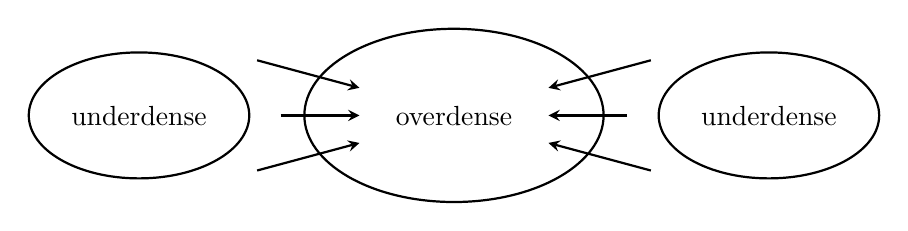
\begin{tikzpicture}[x=1cm,y=1cm,>=stealth]
\draw[thick] (-4,0) ellipse (1.4 and 0.8);
\draw[thick] (0,0) ellipse (1.9 and 1.1);
\draw[thick] (4,0) ellipse (1.4 and 0.8);
\node at (-4,0) {underdense};
\node at (0,0) {overdense};
\node at (4,0) {underdense};
\draw[->,thick] (-2.2,0) -- (-1.2,0);
\draw[->,thick] (2.2,0) -- (1.2,0);
\draw[->,thick] (-2.5,0.7) -- (-1.2,0.35);
\draw[->,thick] (2.5,0.7) -- (1.2,0.35);
\draw[->,thick] (-2.5,-0.7) -- (-1.2,-0.35);
\draw[->,thick] (2.5,-0.7) -- (1.2,-0.35);
\end{tikzpicture}
\caption{A schematic version of the lecture's point about gravitational instability: matter is drawn out of underdense regions and into overdense ones, so small inhomogeneities grow rather than diffuse away.}
\end{figure}

Therefore the universe had to be much more homogeneous in the past than it is now. Yet it could not have been \emph{exactly} homogeneous, for then it would have remained exactly homogeneous and no galaxies would ever have formed. The lecture introduces the dimensionless measure of lumpiness
\begin{equation}
\frac{\delta \rho}{\rho},
\end{equation}
where \(\delta\rho\) is the characteristic excess density of a lump above the background. By running the theory backward, early cosmologists estimated that at decoupling this number had to be of order
\begin{equation}
\frac{\delta \rho}{\rho}\sim 10^{-5}.
\end{equation}

Again the important thing is not that we know why the number is \(10^{-5}\); the lecture explicitly says we do not. The important thing is that there \emph{is} a number. Once that is known, the homogeneity problem becomes sharp.

The inflationary answer, in broad outline, is that the universe expanded by an enormous factor and stretched whatever initial roughness it had so thin that on the observable scales it became extraordinarily smooth. Susskind uses the image of blowing up a crinkled balloon: expansion stretches and flattens. But he is careful not to overdo the analogy, and he does not yet launch into the full inflationary formalism. Instead he turns to the one ingredient he wants us to have in hand for next time: friction.

\paragraph{The falling stone.}
Take a stone moving through a viscous fluid, and call its vertical coordinate \(\phi\). This is a slightly perverse notation for the height of a stone, as Susskind says, but it is the right notation for the field that will soon replace the stone. Suppose the potential energy is \(V(\phi)\). Then the force is
\begin{equation}
F=-\frac{dV}{d\phi}.
\end{equation}

\begin{figure}
\centering

\includegraphics[width=0.72\textwidth]{lecture_08_figure_06.png}
\caption{Potential and force in the blackboard setup for the falling-stone analogy. This is the visual bridge from ordinary mechanics to the inflaton equation of motion.}
\end{figure}

If we take the mass to be \(1\), the frictionless equation is simply
\begin{equation}
\ddot{\phi}=F.
\end{equation}
To model viscosity we add a drag force proportional to velocity and opposite to the motion. With the sign convention that \(\phi\) increases upward, a downward force has \(F<0\), and a stone moving downward has \(\dot\phi<0\). The cleaned equation is therefore
\begin{equation}
\ddot{\phi}+\gamma \dot{\phi}=F,
\end{equation}
where \(\gamma>0\) is the drag coefficient. When the acceleration has died away, the motion approaches terminal velocity:
\begin{equation}
\dot{\phi}_{\mathrm{term}}=\frac{F}{\gamma}.
\end{equation}
Because \(F<0\) for downward motion, the terminal velocity is negative, exactly as it should be.

\begin{figure}
\centering
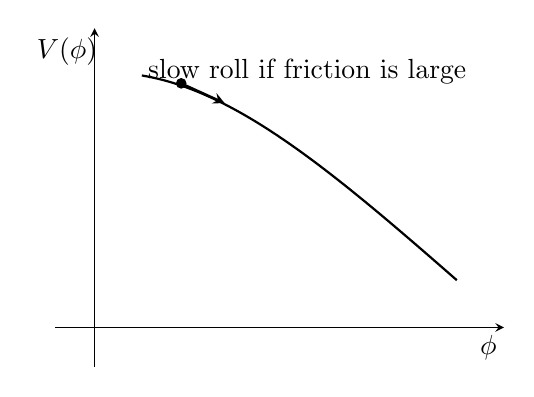
\begin{tikzpicture}[x=1cm,y=1cm,>=stealth]
\draw[->] (-0.5,0) -- (5.2,0);
\draw[->] (0,-0.5) -- (0,3.8);
\draw[thick] (0.6,3.2) .. controls (1.8,3.0) and (3.0,2.0) .. (4.6,0.6);
\node at (5.0,-0.25) {$\phi$};
\node at (-0.35,3.5) {$V(\phi)$};
\filldraw (1.1,3.1) circle (0.06);
\draw[->,thick] (1.1,3.1) -- (1.65,2.85);
\node at (2.7,3.25) {slow roll if friction is large};
\end{tikzpicture}
\caption{A shallow potential hill in the cleaned analogy. Large drag keeps the motion slow even when the force points downhill.}
\end{figure}

\paragraph{From particle mechanics to a scalar field.}
The lecture now replaces the stone by a spatially homogeneous scalar field, the inflaton \(\phi(t)\). Because the field is taken to be uniform in space, the spatial-gradient contribution to the energy is dropped. The homogeneous energy density is then, in the standard cleaned form,
\begin{equation}
\rho_\phi=\frac{1}{2}\dot{\phi}^{\,2}+V(\phi).
\end{equation}
To convert density into total energy, we follow the field inside a comoving unit box. Its physical volume is \(a^3(t)\), so the corresponding Lagrangian is
\begin{equation}
L=a^3\!\left(\frac{1}{2}\dot{\phi}^{\,2}-V(\phi)\right).
\end{equation}
Now apply the Euler--Lagrange equation:
\begin{align}
\frac{d}{dt}\left(\frac{\partial L}{\partial \dot{\phi}}\right)&=\frac{\partial L}{\partial \phi},\\
\frac{\partial L}{\partial \dot{\phi}}&=a^3\dot{\phi},\\
\frac{\partial L}{\partial \phi}&=-a^3\frac{dV}{d\phi}.
\end{align}
Therefore
\begin{equation}
\frac{d}{dt}\left(a^3\dot{\phi}\right)=-a^3\frac{dV}{d\phi}.
\end{equation}
Expanding the time derivative gives
\begin{equation}
a^3\ddot{\phi}+3a^2\dot a\,\dot{\phi}=-a^3\frac{dV}{d\phi}.
\end{equation}
Divide by \(a^3\), define the Hubble rate by
\begin{equation}
H=\frac{\dot a}{a},
\end{equation}
and we arrive at the lecture's equation of motion:
\begin{equation}
\ddot{\phi}+3H\dot{\phi}=F,
\qquad
F=-\frac{dV}{d\phi}.
\end{equation}
Equivalently,
\begin{equation}
\ddot{\phi}+3H\dot{\phi}+\frac{dV}{d\phi}=0.
\end{equation}

This is the payoff of the entire friction discussion. The scalar field evolves exactly like the falling stone, except that the viscosity coefficient is now the cosmological quantity \(3H\). Hubble expansion acts as a kind of cosmic friction. If \(H\) is large and the potential is fairly flat, the field rolls only very slowly. That is the threshold of inflation as the lecture leaves it: not yet the full solution, but the precise equation that will be used next time.

\section{Summary}

The lecture is built around two quantitative puzzles. First, the universe contains a baryon excess of only about one part in \(10^8\), and that forces the Sakharov structure upon us: baryon violation, particle-antiparticle asymmetry, and departure from equilibrium. Second, the universe at decoupling was smooth to about one part in \(10^5\), and that forces us to ask how such smoothness arose in a world where gravity amplifies lumps.

The baryogenesis part ends modestly: the structural ingredients are known, but the number \(10^{-8}\) is not calculable from the level of knowledge available in the lecture. The inflation part ends deliberately at the threshold. We are left with a scalar field in a potential, a Hubble friction term, and the equation
\[
\ddot{\phi}+3H\dot{\phi}+\frac{dV}{d\phi}=0.
\]
That is enough machinery to begin inflation properly in the next lecture.